\documentclass[]{article}
\usepackage[T1]{fontenc}
\usepackage{multicol}
\usepackage{graphicx}
\usepackage{listings}
\usepackage{lmodern}
\usepackage{amssymb,amsmath}
\usepackage{ifxetex,ifluatex}
\usepackage{fixltx2e} % provides \textsubscript
% use upquote if available, for straight quotes in verbatim environments
\IfFileExists{upquote.sty}{\usepackage{upquote}}{}
\ifnum 0\ifxetex 1\fi\ifluatex 1\fi=0 % if pdftex
  \usepackage[utf8]{inputenc}
\else % if luatex or xelatex
  \ifxetex
    \usepackage{mathspec}
    \usepackage{xltxtra,xunicode}
  \else
    \usepackage{fontspec}
  \fi
  \defaultfontfeatures{Mapping=tex-text,Scale=MatchLowercase}
  \newcommand{\euro}{€}
\fi
% use microtype if available
\IfFileExists{microtype.sty}{\usepackage{microtype}}{}
\ifxetex
  \usepackage[setpagesize=false, % page size defined by xetex
              unicode=false, % unicode breaks when used with xetex
              xetex]{hyperref}
\else
  \usepackage[unicode=true]{hyperref}
\fi
\hypersetup{breaklinks=true,
            bookmarks=true,
            pdfauthor={},
            pdftitle={},
            colorlinks=true,
            citecolor=blue,
            urlcolor=blue,
            linkcolor=magenta,
            pdfborder={0 0 0}}
\urlstyle{same}  % don't use monospace font for urls
\setlength{\parindent}{0pt}
\setlength{\parskip}{6pt plus 2pt minus 1pt}
\setlength{\emergencystretch}{3em}  % prevent overfull lines
\setcounter{secnumdepth}{0}

\title{Outletify}
\author{Alan Moy\and Jonathan Wehrend\and Austin Glaser\and Drew Vostrejs}
\date{December 7, 2015}

\begin{document}

\maketitle

\section{Project Tracker}
\url{https://trello.com/methodsandtools}

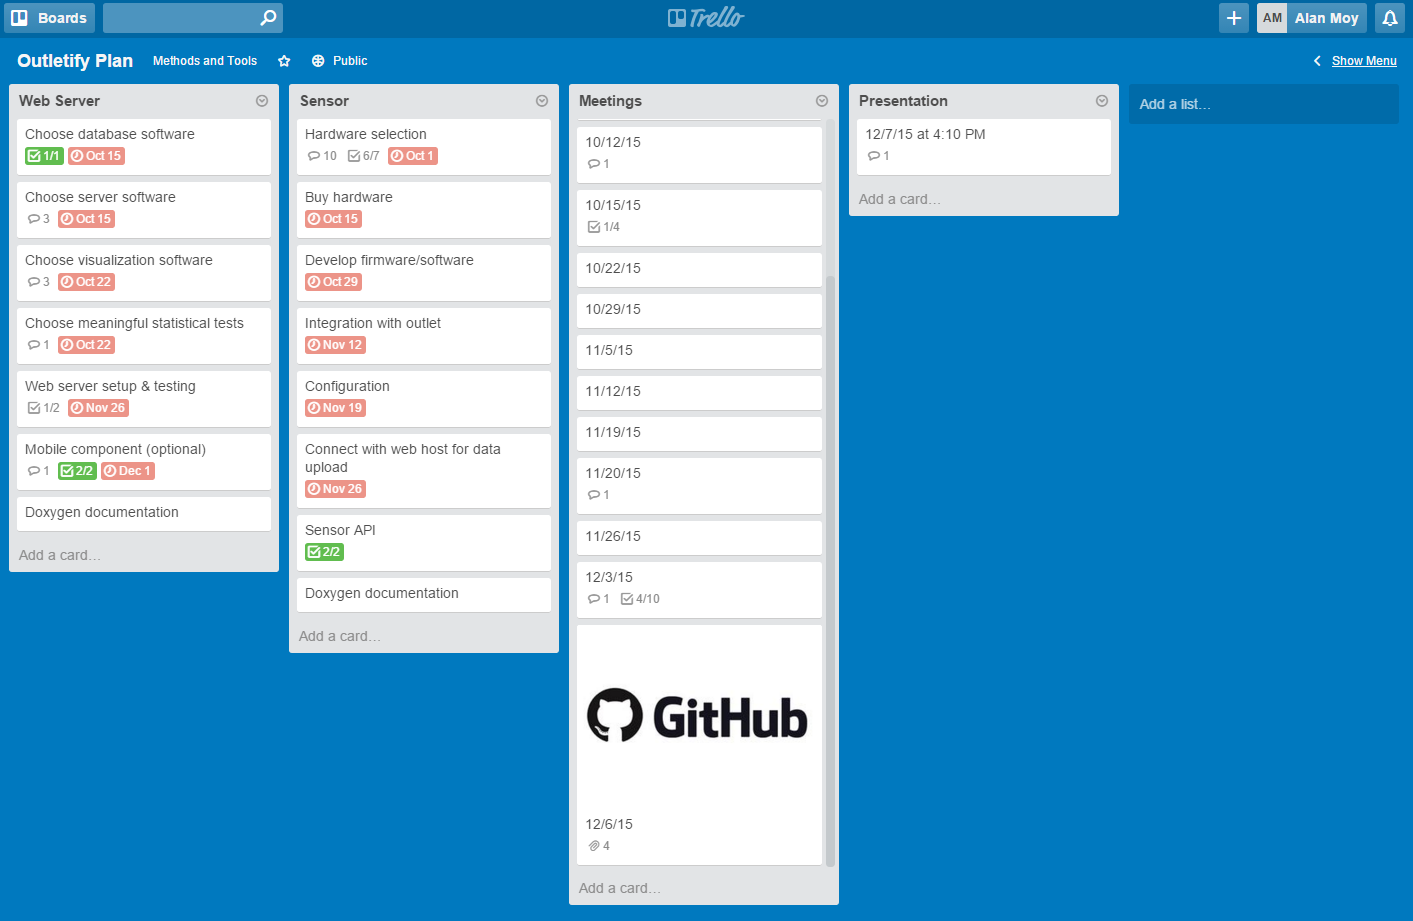
\includegraphics[width=\textwidth]{trello.png}

\section{Video}
\url{https://github.com/austinglaser/csci3308-project/raw/master/Outletify.mp4}

\url{https://youtu.be/muhWIkg7XRw}

\section{VCS}
\url{https://github.com/austinglaser/csci3308-project}

\subsection{Contributions}
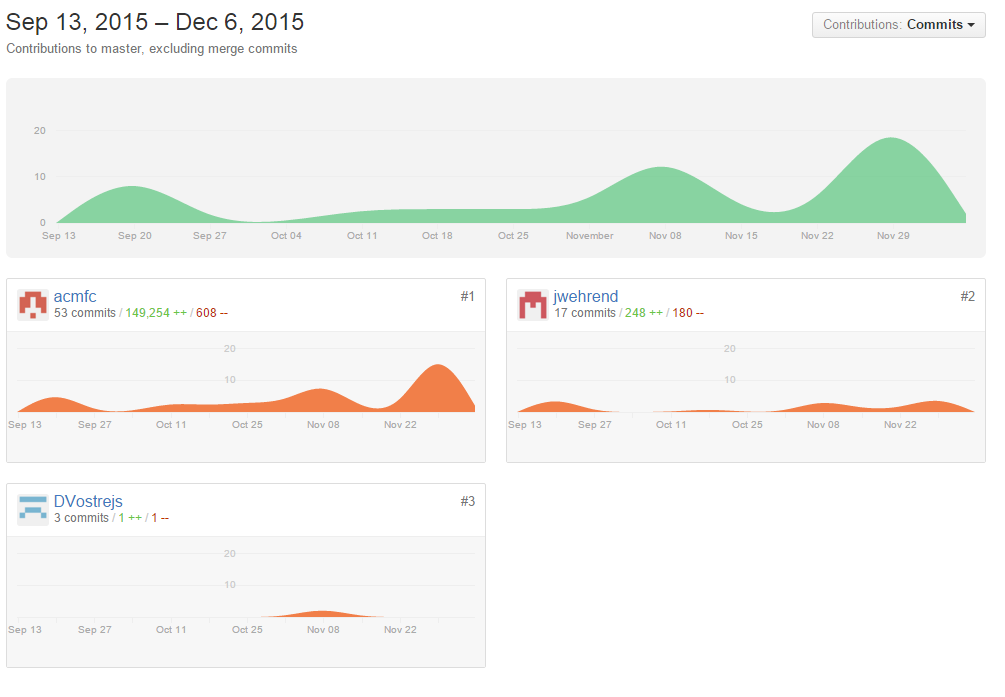
\includegraphics[width=\textwidth]{github_contribution.png}

Alan Moy: acmfc

Jonathan Wehrend: jwehrend

Austin Glaser:

Drew Vostrejs: DVostrejs

The GitHub contributions page does not accurately represent the contributions
of Jonathan Wehrend or Austin Glaser. Austin's commits are not represented at
all. This is probably a result of commiting with an email that is not
associated with his account. Additionally, Only a portion of Jonathan's commits
are represented. Due to an error with git configuration, his commits were made
under a number of different email addresses, including:

jon@engr2-16-108-dhcp.int.colorado.edu \\
jon@engr2-18-171-dhcp.int.colorado.edu \\
jon@engr2-18-59-dhcp.int.colorado.edu \\
jon@Jon-Wehrends-MacBook-Pro.local \\
jon@rgnt1-48-183-dhcp.int.colorado.edu \\
jon@rgnt1-50-164-dhcp.int.colorado.edu \\
jon@rgnt2-113-113-dhcp.int.colorado.edu

The commits associated with some of these emails do not show up on the
contributions page (.local emails are unsupported, for example).

\section{Deployment}
Due to the hardware component of this project, it will not be possible to
deploy the entire project. The server is intended to be run on a Raspberry Pi,
and the sensor is intended to be built and run on a microcontroller that we do
not distribute. However, the server can be installed and run on the CU CS VM
(Fall 2015 edition) with the following steps:

\begin{lstlisting}[breaklines=true, frame=single]
$ git clone https://github.com/austinglaser/csci3308-project.git
$ cd csci3308-project
$ make dep
$ make
\end{lstlisting}

Tests can be run with:

\begin{lstlisting}[breaklines=true, frame=single]
$ make test
\end{lstlisting}

The server can be run with:

\begin{lstlisting}[breaklines=true, frame=single]
$ ./run_server
\end{lstlisting}

When the server is running, the Outletify web site can be accessed at
127.0.0.1:8000.

\section{Auto-Doc}
Doxygen - \url{http://www.stack.nl/~dimitri/doxygen/}

\url{https://github.com/austinglaser/csci3308-project/tree/master/doc/html}

\url{https://github.com/austinglaser/csci3308-project/tree/master/doc/latex}


%\subsection{Theoretical Portion}\label{theoretical-portion}
%\subsubsection{1.}
%Type I error is a false positive---rejecting the null hypothesis when the null
%is actually true. Type II error is the opposite---a failure to reject the null
%hypothesis when it's actually false. It's not possible to minimize them both.
%Lowering one raises the other. A type II error is typically not as bad, since
%it involves no change in the status quo. At worst, it represents a missed
%opportunity.  A type I error, on the other hand, can result in an investment in
%a change that may bring no benefit.
%
%\subsubsection{2.}
%\begin{enumerate}
%\def\labelenumi{(\alph{enumi})}
%
%\item
%  $$ \alpha = 0.02 $$
%  $$ n = 22 $$
%  $$ \bar{x} \pm t_{\alpha/2,n-1} \left( \frac{s}{\sqrt{n}} \right) = \bar{x}
%  \pm 2.518 \left( \frac{s}{\sqrt{n}} \right)$$
%
%\item
%  Assume the data comes from an exponential distribution instead of a normal
%  distribution and use a different test statistic specific to the exponential
%  distribution instead of $t$.
%
%\end{enumerate}
%
%\subsubsection{3.}
%\begin{align*}
%  \mu = 55 \\
%  \sigma = 7
%\end{align*}
%
%\begin{enumerate}
%\def\labelenumi{(\alph{enumi})}
%
%\item
%  $$ \frac{45 - 55}{\sigma} = z = -1.43 $$
%  $$ \Phi \left( -1.43 \right) = 1 - \Phi \left( 1.43 \right) = 0.0764 $$
%\item
%  $$ z_1 = \frac{50 - 55}{\sigma} = -.71 $$
%  $$ z_2 = \frac{70 - 55}{\sigma} = 2.14 $$
%  $$ \Phi \left( 2.14 \right) - \Phi \left( -.71 \right) = \Phi \left( 2.14
%  \right) - \left(1 - \Phi \left( .71 \right)\right)  = 0.9838 - (1 - 0.7611) =
%  0.7449 $$
%\item
%  $$ \Phi \left( z \right) = 0.35 $$
%  $$ 1 - \Phi \left( z \right) = 0.65 $$
%  $$ \Phi \left( -z \right) = 0.65 $$
%  $$ -z = 0.385 $$
%  $$ z = -0.385 $$
%  $$ z \times \sigma = -2.695 $$
%  $$ 55 - 2.695 = 52.305 $$
%\item
%  \begin{align*}
%    n &= 20 \\
%    \bar{x} &= 52 \\
%    \mu &= 55 \\
%    s &= 7 \\
%    \sigma &= 7 \\
%    \alpha &= 0.05 \\
%    H_0: \mu &= 55 \\
%    H_a: \mu &< 55 \\
%    z &= \frac{\bar{x}-\mu_0}{\frac{\sigma}{\sqrt{n}}} = -1.91663 \\ % \text{\hfill \sigma is known, and the data is from a normal distribution} \\
%    \text{P-value} &= P(z < -1.91663) = 0.028
%  \end{align*}
%  Since $0.028 < 0.05$, there is sufficient evidence to reject the null hypothesis.
%\item
%  The probability of a type I error is $\alpha = 0.05$.
%\item
%  We reject $H_0$ if:
%  $$ \frac{\bar{x}-\mu_0}{\frac{\sigma}{\sqrt{n}}} < z_\alpha = -1.645 $$
%  $$ \bar{x} - \mu_0 < -1.645 \left( \frac{\sigma}{\sqrt{n}} \right) $$
%  $$ \bar{x} < -1.645 \left( \frac{\sigma}{\sqrt{n}} \right) + \mu_0 = 52.425 $$
%  The probability of a type II error is:
%  $$ P \left( \bar{x} > 52.425 \right) $$
%  $$ P \left( z > \frac{52.425-53}{\frac{7}{\sqrt{20}}} \right) $$
%  $$ \Phi \left( -\frac{52.425-53}{\frac{7}{\sqrt{20}}} \right) = 0.643 $$
%
%\end{enumerate}
%
%\subsection{Computational Portion}\label{computational-portion}
%
%\subsubsection{1.}
%
%\begin{enumerate}
%\def\labelenumi{(\alph{enumi})}
%
%\item
%\begin{lstlisting}[breaklines=true, frame=single]
%data1 = scan(''HW4ALDdata.txt'')
%hist(data1, xlab=''Accuracy'', main=''Frequency of ALD Accuracy Measurements'')
%\end{lstlisting}
%\includegraphics[width=\textwidth]{comp-1a.eps}
%The data does not look to be very close to normally distributed. But because we
%have more than 40 samples, we can run hypothesis tests anyway because of the
%Central Limit Theorem.
%
%\item
%\begin{lstlisting}[breaklines=true, frame=single]
%u0 = 1
%x = mean(data1)
%s = sd(data1)
%n = length(data1)
%z = (x - u0)/(s/sqrt(n))
%# Can we reject the null?
%z < qnorm(0.05)
%[1] TRUE
%\end{lstlisting}
%The data does provide strong evidence that the true average ALD is less than
%1.0 at a 5\% significance level.
%
%\item
%\begin{lstlisting}[breaklines=true, frame=single]
%pval = pnorm(z)
%pval
%[1] 1.093775e-08
%\end{lstlisting}
%
%\end{enumerate}
%
%\subsubsection{2.}
%
%\begin{enumerate}
%\def\labelenumi{(\alph{enumi})}
%
%\item
%\begin{lstlisting}[breaklines=true, frame=single]
%data2 = scan(''HW4Radondata.txt'')
%hist(data2, xlab=''Radon measurement in pCi/L'', main=''Frequency of Radon Measurements'')
%\end{lstlisting}
%\includegraphics[width=0.7\textwidth]{comp-2a.eps}
%
%\item
%Use a t test because the data appears to be normally distributed and there are
%only 12 samples.
%
%$H_0: \mu = 100$ \\
%$H_a: \mu \ne 100$
%\begin{lstlisting}[breaklines=true, frame=single]
%u0 = 100
%x = mean(data2)
%s = sd(data2)
%n = length(data2)
%t = (x - u0)/(s/sqrt(n))
%# Can we reject the null?
%t < qt(0.025, df=n-1)
%[1] FALSE
%\end{lstlisting}
%The data does not provide strong evidence that the reading differs from 100.
%
%\item
%\begin{lstlisting}[breaklines=true, frame=single]
%pval = pt(t, df=n-1)
%pval
%[1] 0.4064447
%\end{lstlisting}
%
%\end{enumerate}
%
%\subsubsection{3.}
%
%\begin{enumerate}
%\def\labelenumi{(\alph{enumi})}
%
%\item
%\begin{lstlisting}[breaklines=true, frame=single]
%p0 = .39
%q0 = 1 - p0
%n = 150
%alpha = 0.01
%n * p0 > 10
%[1] TRUE
%n * q0 > 10
%[1] TRUE
%p = 72/150
%z = (p - p0)/sqrt(p0*q0/n)
%# Can we reject the null?
%z > qnorm(1 - alpha/2)
%[1] FALSE
%\end{lstlisting}
%The data does not provide strong evidence the actual percentage of type A
%donations differs from 39\%.
%
%\item
%\begin{lstlisting}[breaklines=true, frame=single]
%# Could we have rejected the null with significance level .05?
%z > qnorm(1 - 0.05/2)
%[1] TRUE
%\end{lstlisting}
%If a significance level of 0.05 had been used, the test would have rejected
%$H_0$.
%
%\end{enumerate}
%
%\subsubsection{4.}
%\begin{lstlisting}[breaklines=true, frame=single]
%data4 = read.table(''HW4Fabricdata.txt'', header=TRUE)
%diff = data4$U - data4$A
%x = mean(diff)
%s = sd(diff)
%t = (x - 0)/(s/sqrt(8))
%n = 8
%# Can we reject the null?
%t > qt(1 - 0.01, df=n - 1)
%[1] FALSE
%\end{lstlisting}
%The test failed to reject the null hypothesis.

\end{document}
